% Created 2024-06-25 Tue 16:19
% Intended LaTeX compiler: pdflatex
\documentclass[10pt,a4paper,onecolumn,notitlepage,oneside,dvipdfmx]{article}
\usepackage{graphicx}
\usepackage{longtable}
\usepackage{wrapfig}
\usepackage{rotating}
\usepackage[normalem]{ulem}
\usepackage{amsmath}
\usepackage{amssymb}
\usepackage{capt-of}
\usepackage{hyperref}
\usepackage[newfloat]{minted}
\usepackage{fancyhdr}
\usepackage{amsmath}
\usepackage{amssymb}
\usepackage{bm}
\usepackage{color}
\usepackage{graphicx}
\usepackage{tikz}
\usepackage{wrapfig}
\setlength{\oddsidemargin}{-10mm}
\setlength{\topmargin}{-10mm}
\setlength{\textheight}{245mm}
\setlength{\textwidth}{180mm}
\renewcommand{\figurename}{Fig.}
\renewcommand{\tablename}{Tab.}
\newcommand{\Figure}[1]{\figurename{\ref{#1}}}
\newcommand{\Table} [1]{\tablename {\ref{#1}}}
\makeatletter
\newcommand{\figcaption}[1]{\def\@captype{figure}\caption{#1}}
\newcommand{\tblcaption}[1]{\def\@captype{table}\caption{#1}}
\pagestyle{fancy}
\lhead{\@leftheader}
\rhead{\@rightheader}
\newcommand{\leftheader} [1]{\def\@leftheader{#1}}
\newcommand{\rightheader}[1]{\def\@rightheader{#1}}
\leftheader{グループゼミ資料}
\rightheader{Ver.Ka}
\renewcommand{\maketitle}{%
\begin{center}{\Large \@title}\end{center}%
\begin{flushright}\@author\\ \@date\end{flushright}%
\hrulefill\\}
\usepackage{multirow}
\usepackage{subcaption}
\usepackage{lscape}
\usepackage{ascmac}
\usepackage{bm}
\usepackage{here}
\usepackage{latexsym}
\usepackage{algorithm}
\usepackage{algpseudocode}
\usepackage{url}
\usetikzlibrary{arrows,automata}
\algnewcommand\algorithmicforeach{\textbf{for each}}
\algdef{S}[FOR]{ForEach}[1]{\algorithmicforeach\ #1\ \algorithmicdo}
\DeclareMathOperator*{\argmax}{arg\,max}
\DeclareMathOperator*{\argmin}{arg\,min}
\author{Vincent Conus}
\date{2024/06/19}
\title{Ender-3 S1 Pro: 使う方法ガイド\\\medskip
\large 稲垣研究室、南山大学}
\hypersetup{
 pdfauthor={Vincent Conus},
 pdftitle={Ender-3 S1 Pro: 使う方法ガイド},
 pdfkeywords={},
 pdfsubject={},
 pdfcreator={Emacs 30.0.50 (Org mode 9.6.15)}, 
 pdflang={English}}
\begin{document}

\maketitle
\tableofcontents

\section{初めに}
\label{sec:orgbd3cd64}
Crealityの「Ender-3 S1 Pro」\footnote{\url{https://www.creality.com/products/creality-ender-3-s1-pro-fdm-3d-printer}}と言うの機会は様々な種類のポリマー材料を用いて印刷できる積層造形装置です。

\begin{figure}[htbp]
\centering
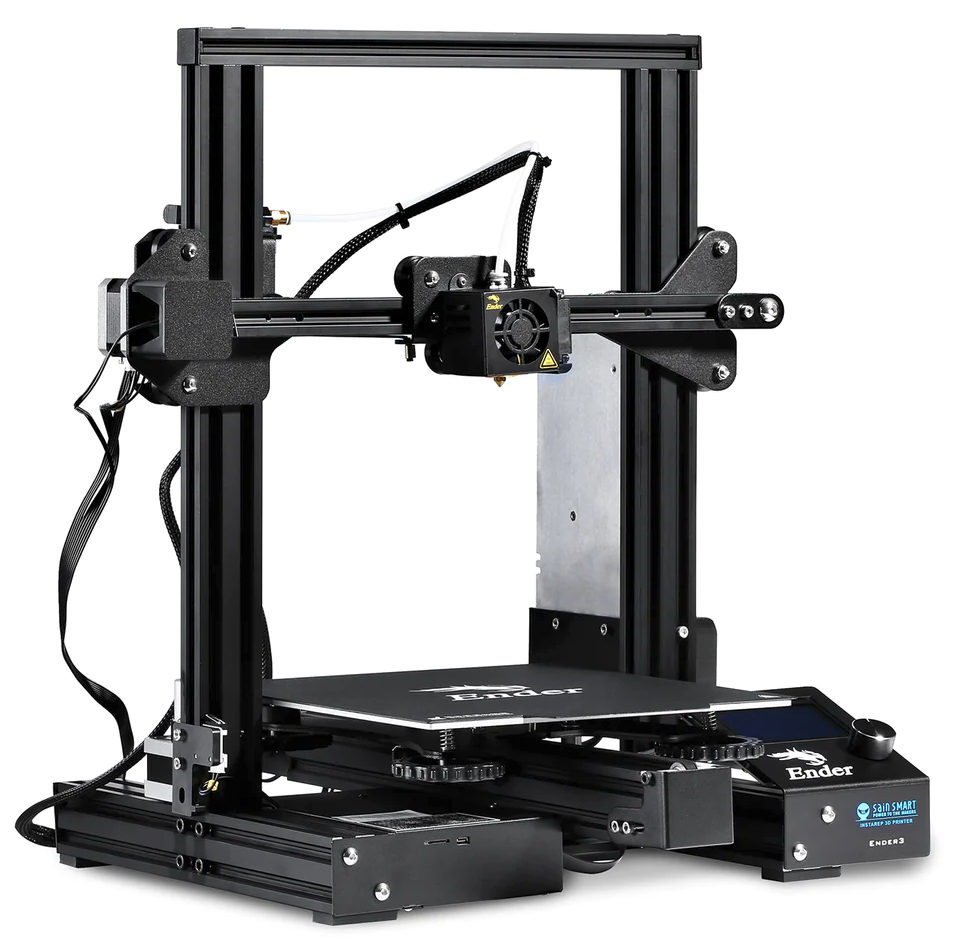
\includegraphics[width=0.65\textwidth]{img/ender3.png}
\end{figure}

\subsection{練習:Benchy}
\label{sec:org476461c}
このガイドにBenchyと言うモデルは練習をしましょう。そのモデルを使うと、色々な問題を知ります:
\begin{itemize}
\item 小さなベースは、ベッドの接着をテストすることができます。
\item キャビン部分は、アーチや橋、小さなディテールをテストすることができます。
\item 船体は、はみ出し具合をテストしたり、印刷の平滑性の欠点を見ることができます
\item 小さくてかわいいので、もっとたくさん作りたくなります!
\end{itemize}
\begin{figure}[htbp]
\centering
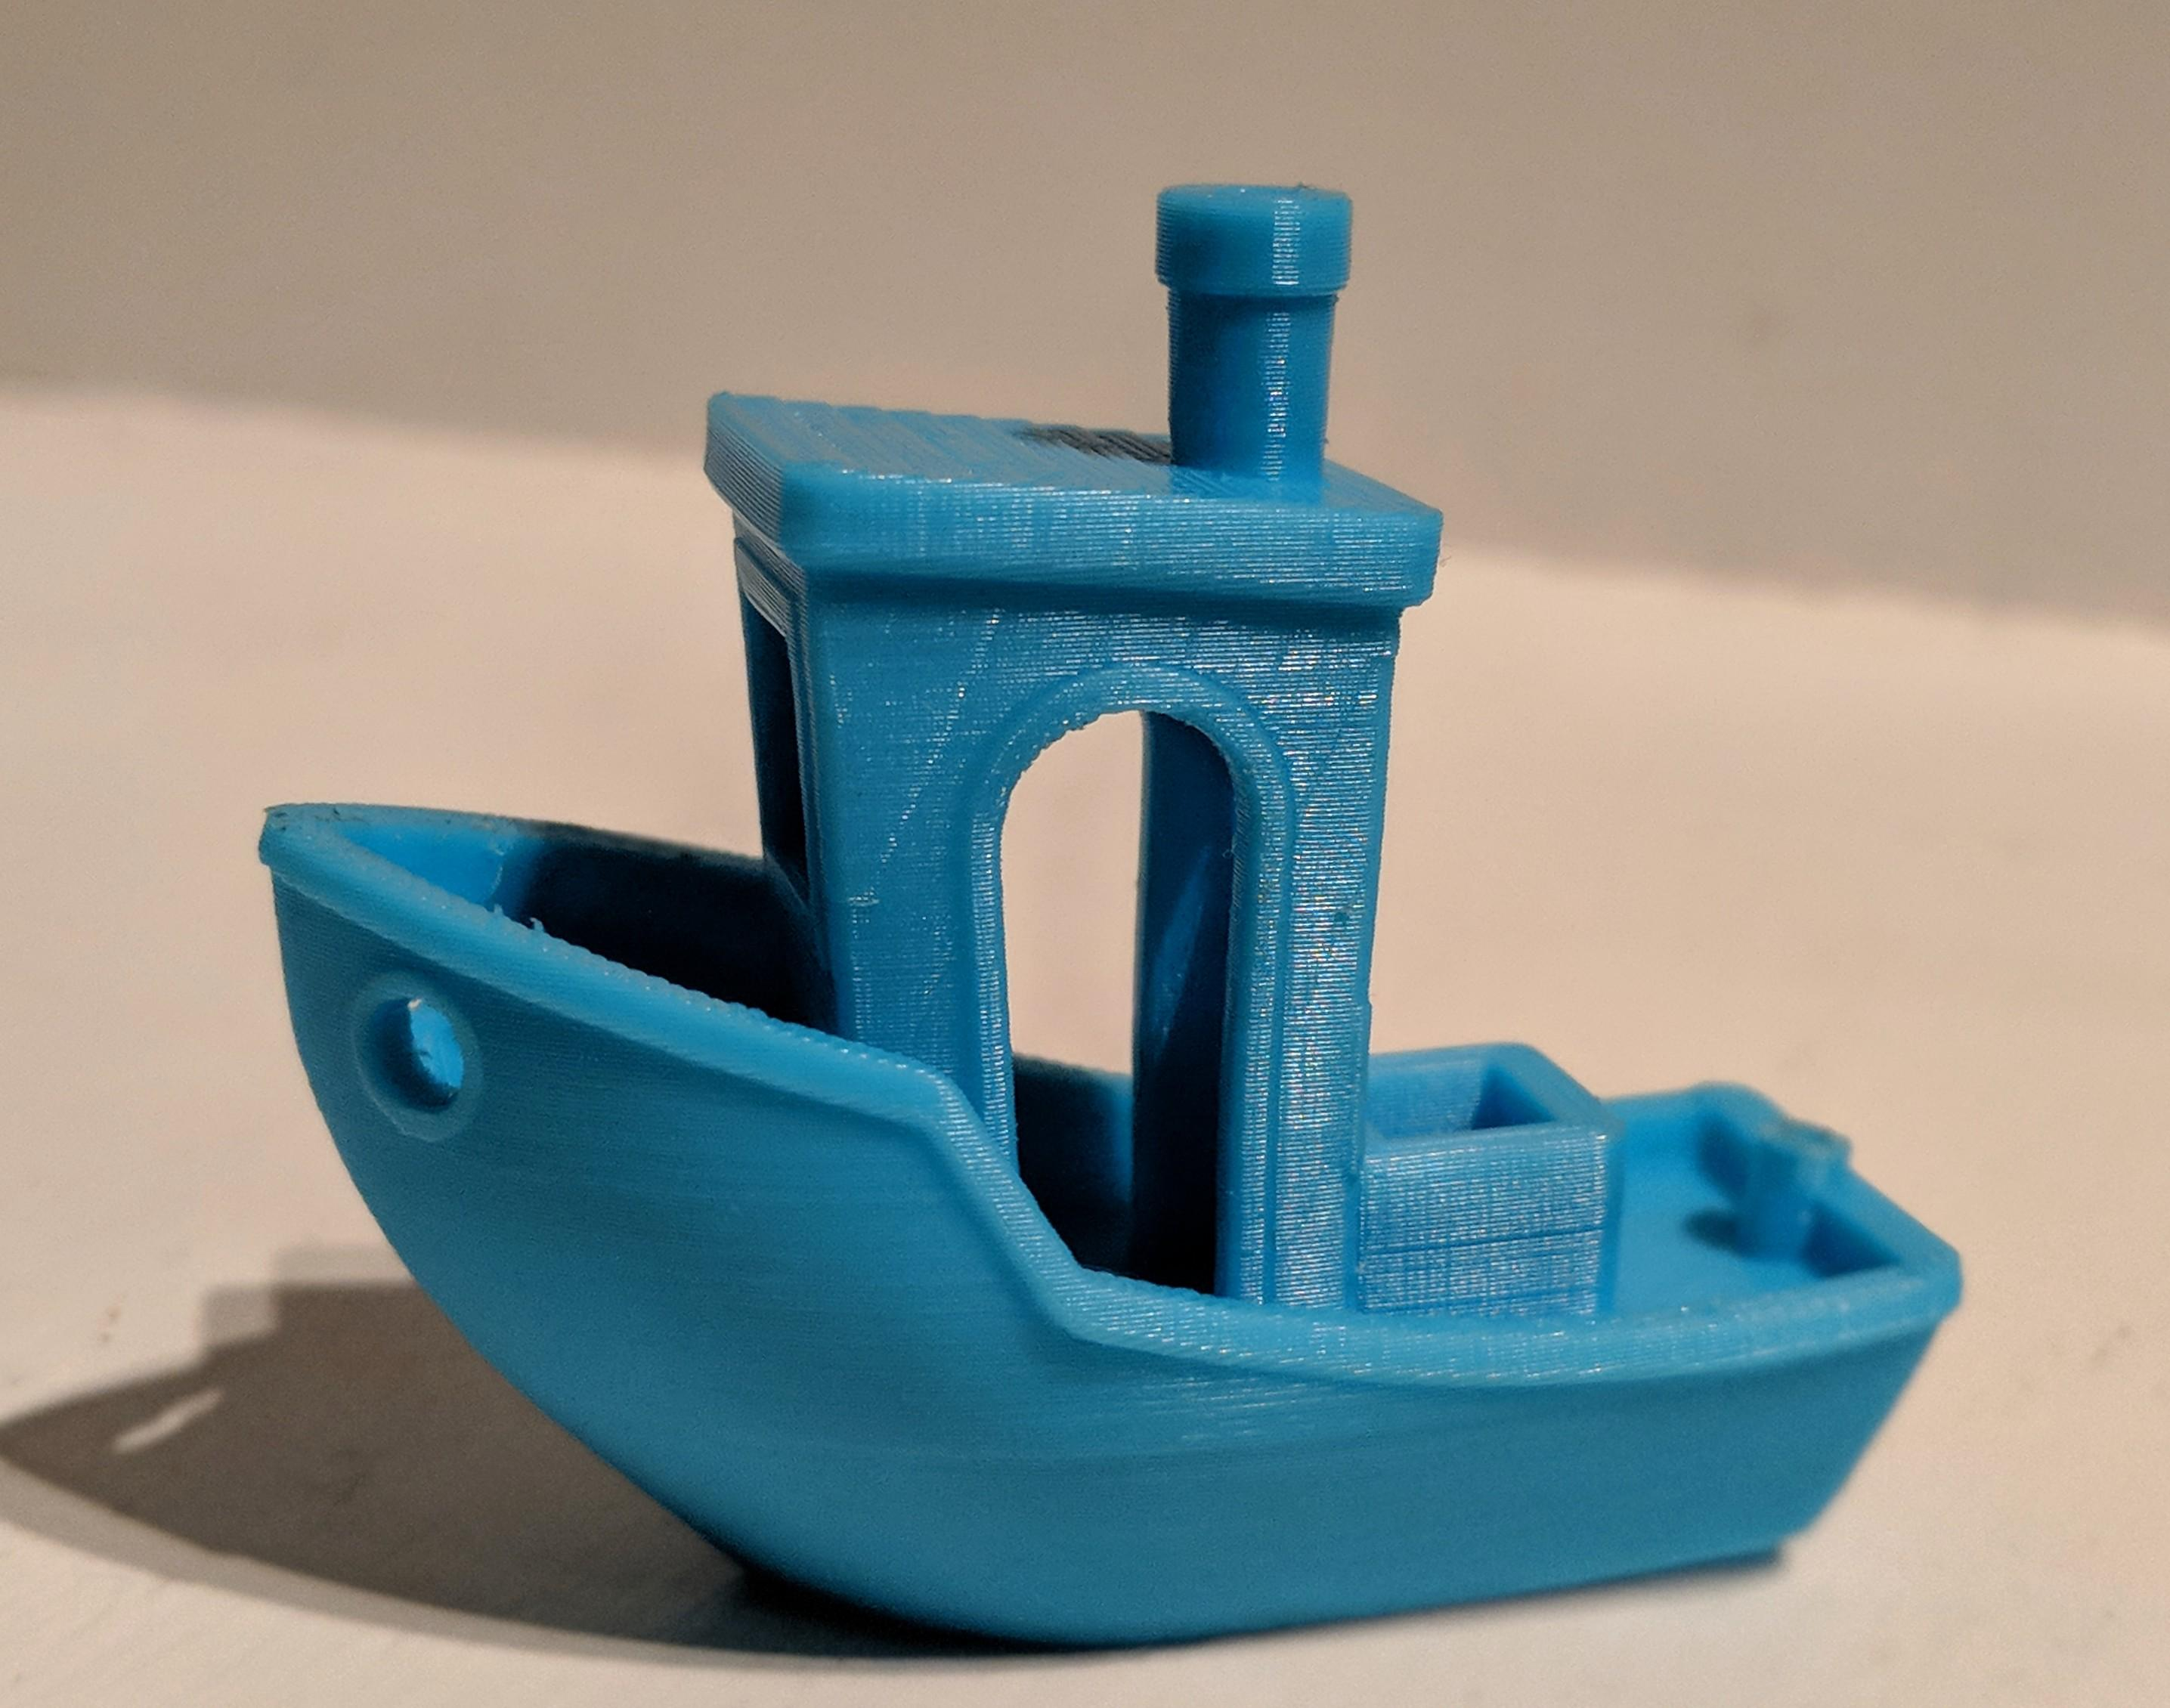
\includegraphics[width=0.65\textwidth]{img/benchy.jpg}
\caption{終わった船のプリント。プリントの層をみえる。}
\end{figure}

BenchyのSTLファイルはオンラインにドーンロードができます。
\begin{itemize}
\item Prusa Printables: \url{https://www.printables.com/model/3161-3d-benchy/files}
\item Thingivers: \url{https://www.thingiverse.com/thing:763622/files}
\end{itemize}

色々なファイルが見られるんですが、欲しいのは「3dbenchy.stl」と言うのです。


\section{スライシング}
\label{sec:orgfdcbba2}
3Dモデルが作成または取得された場合、そのファイルをプリンターで理解できるようにす
るために「スライス」する必要があります。

スライス処理では、3Dモデル(通常はSTL形式)を入力として受け取り、プリンタヘッド
がパーツを描画するためにたどるパスを直接表す座標のリストを作成します。プリンタヘッ
ドの速度やプリンタの温度設定など、その他の情報も含まれます。

\subsection{練習}
\label{sec:org6f97c04}

\section{プリンチング}
\label{sec:org9e0b062}
\subsection{練習}
\label{sec:orgf567e1e}

\section{整備助言}
\label{sec:org9be53e5}

\subsection{湿気}
\label{sec:orgc54b4ad}
3Dプリンター用ラメントスプールは、一般的に湿気に弱い。
もし長期間使用しない場合は、プリンターから取り出して箱に戻し、理想的にはケイ酸塩を入れた袋を中に入れて保管してください。
\end{document}
